\documentclass[11pt, conference]{IEEEtran}
\IEEEoverridecommandlockouts
% The preceding line is only needed to identify funding in the first footnote. If that is unneeded, please comment it out.
\usepackage{algorithm}
\usepackage{algpseudocode}

\usepackage{cite}
\usepackage{amsmath, amsfonts, amsthm, amssymb} 
% \usepackage{algorithmic}
\usepackage{subfigure}
\usepackage{placeins}
\usepackage{graphicx}
\usepackage{textcomp}
\usepackage{xcolor}
\usepackage{lipsum}
\usepackage{hyperref}
\usepackage{float}
\usepackage{multirow}
% \usepackage{subcaption}
\usepackage[OT1]{fontenc} 
% \usepackage{fontawesome5}
\algrenewcommand\algorithmicrequire{\textbf{Input:}}
\algrenewcommand\algorithmicensure{\textbf{Output:}}

\usepackage{enumitem} % enumerate / ordered list
\usepackage{booktabs} % three-line table
\usepackage{array}   % for \newcolumntype macro
\usepackage{listings} % MATLAB code block
\usepackage{pdfpages} % include external pdf pages
\usepackage[bottom]{footmisc} % move footnote to the bottom
\usepackage{mathtools}
\newcolumntype{C}{>{$}c<{$}} % math-mode version of "l" column type

\theoremstyle{definition} % definition
\newtheorem{definition}{Definition}[section]
\newtheorem{theorem}{Theorem}[section]
\newtheorem{remark}{Remark}[section]

\newcommand{\dd}{\mathrm{d}}
\newcommand{\RR}{\mathbb{R}}
\newcommand{\NN}{\mathbb{N}}
\newcommand{\ZZ}{\mathbb{Z}}
\newcommand{\CC}{\mathbb{C}}
\newcommand{\PP}{\mathbb{P}}


\hypersetup{
    colorlinks,
    linkcolor={black},
    citecolor={black},
    urlcolor={blue!80!blue}
}
\def\BibTeX{{\rm B\kern-.05em{\sc i\kern-.025em b}\kern-.08em
    T\kern-.1667em\lower.7ex\hbox{E}\kern-.125emX}}
\begin{document}

\title{LocoJump: Controlled Versatile Jumping from Locomotion of Quadruped Robot
\thanks{This is the report for course ROB 590 Direct Study advised by Professer Yanran Ding.}%
}

\author{
\IEEEauthorblockN{Yulun Zhuang}
\IEEEauthorblockA{\textit{Robotics} \\
\textit{University of Michigan}\\
Ann Arbor, United States \\
yulunz@umich.edu}
}

\maketitle

% \begin{abstract}
% % TODO
% \end{abstract}

\begin{IEEEkeywords}
Legged Locomotion, Trajectory Optimization, Reinforcement Learning
\end{IEEEkeywords}


\section{Introduction}
% Provide background and motivation of the project. Motivate why the problem you are solving is important. What applications require this kind of method?
% State a concrete project goal.
% Conduct a comprehensive review of existing literature, focusing on recent advancements and state-of-the-art.

\subsection{Background}
The agile locomotion capabilities (e.g. parkour in Figure \ref{fig:parkour_atlas}) of legged robots are of vital important yet highly challenged for applications like search and rescue. With the recent advancement in Reinforcement Learning (RL), its application in legged robot control has shown promising result to generate highly dynamic and robust locomotion policies. This project focuses on utilizing the state-of-the-art toolboxes to train RL aided model-based control policies for legged robots in simulation.


\begin{figure}[htb]
    \centering
        \textsf{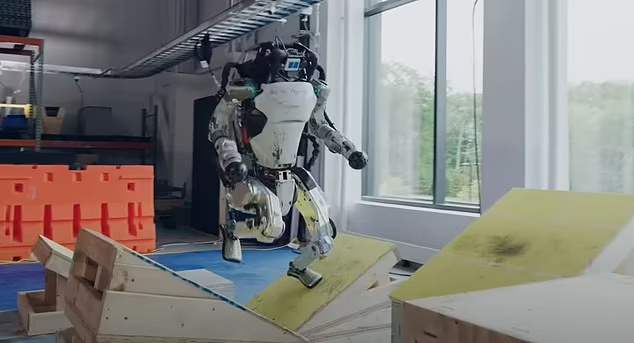
\includegraphics[width=0.9\columnwidth]{figures/parkour_atlas.png}}
        \caption{The parkour motion performed by Atlas Robot}
        \label{fig:parkour_atlas}
\end{figure}


\subsection{Related Works}

\begin{itemize}
    \item Optimized jumping of quadruped\cite{nguyen2019optimized}
    \item Running jump via online optimization\cite{chignoli2021online}
    \item Continuous jumping via MPC\cite{nguyen2022continuous}
    \item Robust quadruped jumping via deep RL\cite{bellegarda2020robust}
    \item Continuous jumping via relaxed centroidal QP\cite{yang2023cajun}
    \item Jumping via learned acceleration residual\cite{yang2023continuous}
    \item Learning aided centroidal QP locomotion\cite{xie2022glide}
\end{itemize}

\subsection{Objectives}
Enable the parkour capability of versatile jumping from running on a Unitree Go2 quadruped robot via RL assisted model-based control.
\begin{itemize}
    \item {Assumptions}: Given desired landing states and contact schedule for jumping
    \item {Planning}: Heuristic acceleration planner by authoring vertical component of acceleration
    \item {Tracking}: Centroidal QP with learned residuals of reference
    
\end{itemize}


\begin{figure*}
    \centering
    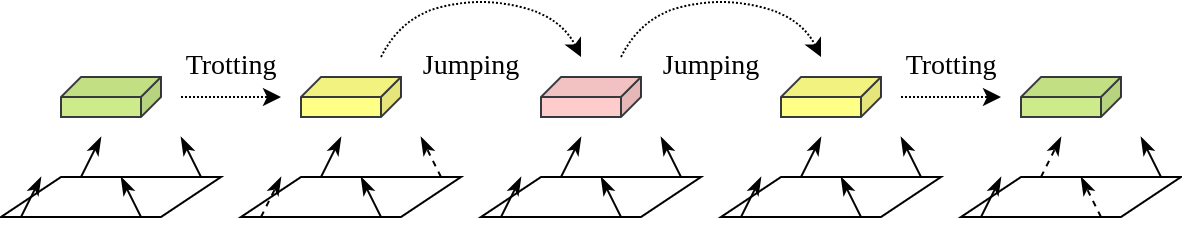
\includegraphics[width=0.9\textwidth]{figures/parkour.png}
    \caption{A nominal parkour case in sagittal plane with controlled versatile jumping from trotting of a quadruped robot modeled as SRB}
    \label{fig:parkour}
\end{figure*}


\section{Reference Trajectory Generation}
% Problem formulation: robot modeling, optimization formulation
% Walk through the methodologies used to solve the problem.
% Describe, in detail, using equations and illustrations where necessary, what you did to implement your project. 
% A block diagram showing the steps involved in the method is very helpful. 
% Make sure to discuss why you made the decisions you did.

The transitions primarily investigated and optimized in this project are between jumping and running where the jumping and running gaits are chosen to be pronking and trotting respectively.

The reference trajectory for pronking and trotting are designed separately and parameterized by center-of-mass (COM) initial position ($p_0$), velocity ($v_0$) and target position ($p_d$) for each sequence of motion, while the transition between them are optimized individually. The main reason behind this design is that a complete reference trajectory can be automatically generated by random sampling given the number of sequence, since each reference motion can be connected with each other in arbitrary orders while continuity is ensured by optimizing transitions between them.

Note that the reference motion are designed in sagittal plane ($x$-$z$) of the robot for simplicity, but the robot are fully unconstrained in $\RR^3$ during simulation.

\subsection{Robot Modeling}
Due to the nature of chosen gaits, the body of the quadruped robot are designed to remain upright during each gait, and the mass of four legs are small enough to be ignored compared to body. Therefore, the robot model is simplified as a single rigid-body (SRB, Figure \ref{fig:robot_model}). Consequently, the joint level dynamics and kinematics of the robot are not included in the optimization.

The state of the SRB model of the robot is given by
\begin{align}
    \mathbf{x} = [\mathbf{p}\ \boldsymbol{\Theta}\ \mathbf{v}\ {^\mathcal{B}\boldsymbol{\omega}}]^T
\end{align}
where $\mathbf{p}\in\RR^3$ is the position of COM, $\boldsymbol{\Theta}\in\RR^3$ is the orientation of the SRB represented by Euler angles, $\mathbf{v}\in\RR^3$ is the velocity of the COM, and $\boldsymbol{\omega}\in\RR^3$
is the angular velocity of the SRB represented in the body frame $\mathcal{B}$.

The state $\mathbf{x}$ is controlled via the net external wrench applied on the robot’s COM via the reaction forces
at the feet. The SRB dynamics is given by
\begin{align}
    \begin{bmatrix}
        m\ddot{\mathbf{p}}\\
        {^\mathcal{B}\mathbf{I}}\dot{\boldsymbol{\omega}}
    \end{bmatrix}
    = \sum_{i=0}^{n}
    \begin{bmatrix}
        \mathbf{f}_i + \mathbf{g}\\
        \mathbf{r}_i\times\mathbf{f}_i
    \end{bmatrix}
\end{align}
where $\mathbf{f}_i\in\RR^3$ the force at foot $i$, $\mathbf{r}_i\in\RR^3$ the vector point from the position of foot $i$ to COM, and $n$ the number of feet in contact.

\begin{figure}[htb]
    \centering
        \textsf{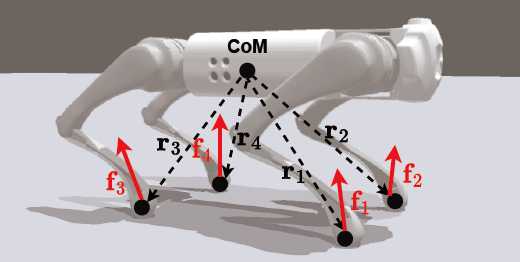
\includegraphics[width=0.7\columnwidth]{figures/robot_model.png}}
        \caption{SRB model representations on Go1 robot}
        \label{fig:robot_model}
\end{figure}

\subsection{Pronking Trajectory}
The projectile motion equations are used to determine the state at liftoff that produces the desired CoM trajectory throughout flight, parameterized by the desired final position of the robot, e.g. jumping onto a stair or over a gap.

The desired position of the robot when it touches down $\mathbf{p}^{ref}(t_{TD})\in\RR^3$ is related to the reference trajectory of the robot throughout liftoff via
\begin{align}
    \mathbf{p}^{ref}(t_{TD}) = \mathbf{p}^{ref}(t_{LO}) + \mathbf{v}^{ref}(t_{LO})\Delta t_{FL} + \frac{1}{2}\mathbf{g}\Delta t_{FL}^2
    \label{eqn:projectile}
\end{align}
where $\mathbf{p}^{ref}(t_{LO})\in\RR^3$ and $\mathbf{v}^{ref}(t_{LO})\in\RR^3$ are the position and velocity of the robot when it lifts off the ground, $\Delta t_{FL}$ is the duration of the flight phase, and $\mathbf{g}\in\RR^3$ is the COM acceleration due to gravity.

Since the initial state of the robot is known, the reference position and velocity can be computed by integrating the reference acceleration $\mathbf{a}^{ref}(t)\in\RR^3$ of the robot from zero to the time of liftoff $t_{LO}$.

The reference trajectories is generated by first manually authoring simple trajectories for the vertical component of the reference acceleration, which is similar to\cite{chignoli2021online}. The heuristic used for vertical acceleration is the following.
\begin{align}
    a_z^{ref}(t) = (\beta + \frac{t}{t_{LO}}\gamma)\frac{1}{m} \sum_{i=1}^{n}\phi_i(t)f_{max, i}
\end{align}
where $\beta\in\RR$ and $\gamma\in\RR$ are empirical scaling parameters and $\phi_i(t)\in [0, 1]$ indicates whether the $i$th foot is in contact at time $t$.

Using the trajectory of $a_z^{ref}(t)$, the reference trajectories for $v_z^{ref}(t)$ and $p_z^{ref}(t)$ can be obtained via integration from the initial state. Consequently, the vertical component of (\ref{eqn:projectile}) can be solved to obtain the duration of flight $\Delta t_{FL}$, given the landing height of ${p}^{ref}_z(t_{TD})$. Assuming constant acceleration in the forward and lateral directions, the forward and lateral components of (\ref{eqn:projectile}) can be solved to obtain the complete $\mathbf{a}^{ref}(t)$ that result in the robot landing at $\mathbf{p}^{ref}(t_{TD})$. The generated trajectory is shown in Figure \ref{fig:jump_tracking_wo_opt}.

\subsection{Trotting Trajectory}
The major component of a trotting motion is in the forward direction, so a simple trapezoidal velocity profile is designed in $x$ axis while keeping zeros in other directions (Figure \ref{fig:trot_tracking}).


\subsection{Transition Optimization}
As shown in Figure \ref{fig:jump_tracking_wo_opt}, the heuristic jumping reference can not stabilize the robot after landing and prepare it for the next motion. To achieve this, the dynamic system during landing phase can be formulated as a point-mass model subjected to propulsion forces in the sagittal plane (Figure \ref{fig:shooting_diagram}).

\begin{figure}[htb]
    \centering
        \textsf{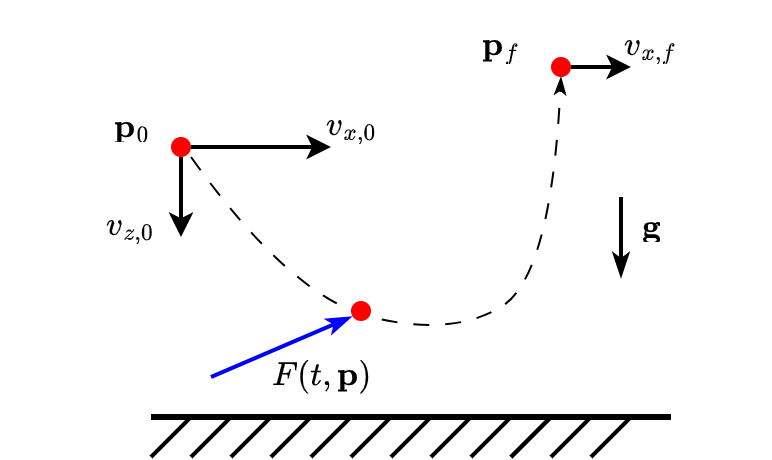
\includegraphics[width=0.7\columnwidth]{figures/traj_opt.png}}
        \caption{Transition from landing state to a stabilized target state}
        \label{fig:shooting_diagram}
\end{figure}

\begin{itemize}
    \item State: $\mathbf{s} = [\mathbf{p}\ \mathbf{v}]^T \in \RR^4$
    \item Control: $\mathbf{a} = \sum^4_{i=0} F_it^i \coloneqq F(t, p)$ \\
    where $\mathbf{p} = [F_0\ F_1\ F_2\ F_3]^T\in \RR^{4\times2}$
    \item Dynamics: $\dot{\mathbf{s}} = [\mathbf{v}\ F(t, \mathbf{p}) - \mathbf{g}]^T \coloneqq f(t, \mathbf{s}, \mathbf{p})$
\end{itemize}

The optimization can be formulated as a nonlinear programming problem (NLP) to find a set of coefficients $\mathbf{p}$ and time to stabilize $t_f$ by minimizing the square some of parameterized ground reaction forces $F(t, \mathbf{p})$ while subjecting to boundary state constraints (\ref{eqn:opt_origin}).
\begin{equation}
    \begin{aligned}
        \min_{\mathbf{p}, t_f} \int_0^{tf}\|&F(t, \mathbf{p})\|^2dt\\
        s.t.\quad\quad &\mathbf{s}(0) = \mathbf{s}_0\\
        &\mathbf{s}(t_f) = \mathbf{s}_d\\
        &\mathbf{s} \in \mathcal{S}
    \end{aligned}
    \label{eqn:opt_origin}
\end{equation}
where $\mathcal{S}$ is the boundary of robot's kinematic limits.

Since the integration upper bound $t_f$ is also a optimization variable, time-transformation could be applied so that the system is integrated over a normalized time interval between $[0, 1]$. Let $\tau = t/t_f$,
\begin{equation}
    \begin{aligned}
        \min_{\mathbf{p}, t_f} \int_0^{1}\|&F(t_f \tau, \mathbf{p})\|^2t_f d\tau\\
        s.t.\quad\quad &\mathbf{s}(0) = \mathbf{s}_0\\
        &\mathbf{s}(1) = \mathbf{s}_d\\
        &\mathbf{s} \in \mathcal{S}
    \end{aligned}
\end{equation}

Therefore, this NLP can be solve via the single shooting method in CasADi\cite{andersson2019casadi}.


\subsection{Training Environment with Reference}

The design of the centroidal policy is to mimic a MPC controller with receding horizon manner, which takes the input of a sequence of future reference states and output the residual of current reference state as a refinement, while minimizing the state tracking errors.

\begin{itemize}
    \item {Observation}: $[\mathbf{x},\ \mathbf{r},\ \mathbf{x}_{1}^{ref}, \dots,\ \mathbf{x}_{n_h}^{ref}]$
    \item {Action}: $[\Delta\mathbf{x}_{1}^{ref}, \Delta\mathbf{r}]$
    \item {Reward}: $\|\mathbf{x} - (\mathbf{x}_{1}^{ref} + \Delta\mathbf{x}_{1}^{ref})\|_{\mathbf{R}}$, e.t.c
\end{itemize}
where the subscript $1$ denotes the index of current time step, $n_h$ is the length of predictive horizon and $\mathbf{R}$ is a diagonal matrix represent the weight of each state dimension.

\section{Experiments and Results}
% Simulation and optimization set up.
% Figures that present numerical simulation results.
% Interpretation of the results.

In this section, the implementation of simulation environment is discussed, and reference tracking curves are presented in Figures \ref{fig:jump_tracking_wo_opt},\ref{fig:jump_tracking_w_opt},\ref{fig:trot_tracking},\ref{fig:continuous_jump},\ref{fig:mix_jump} for both single motion and multiple motions in sequence with or without optimized transitions.

\subsection{Environment Setup}

The experiment environment is setup in Isaac Gym\cite{makoviychuk2021isaac}, a high performance gpu-based physics simulation for robot learning. The codebase is implemented based on a fully paralleled (i.e. operate asynchronously in parallel) model-based quadruped controller framework from CAJun\cite{yang2023cajun}. A novel reference trajectory generator is implemented to rollout a long reference by randomly sampling from a set of primitive motion sequences, and current reference states with a forward horizon are feed into the training environment according to the tracking progress w.r.t each robot in parallel.


\subsection{Single Gait Tracking}

\begin{figure}[htb]
    \centering
        \textsf{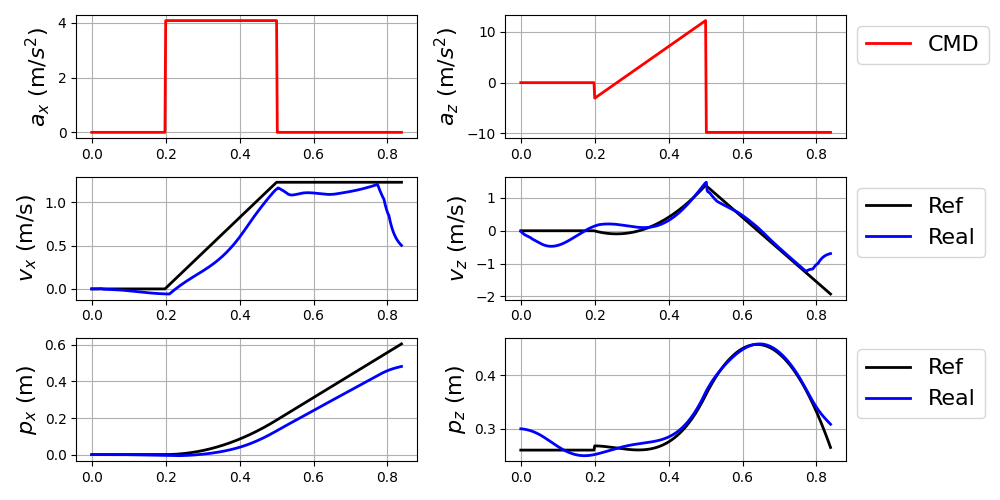
\includegraphics[width=0.85\columnwidth]{figures/jump_wo_opt_tracking.png}}
        \caption{Single pronking circle without optimized transition. The position tracking MSE error is 0.0026.}
        \label{fig:jump_tracking_wo_opt}
\end{figure}

\begin{figure}[htb]
    \centering
        \textsf{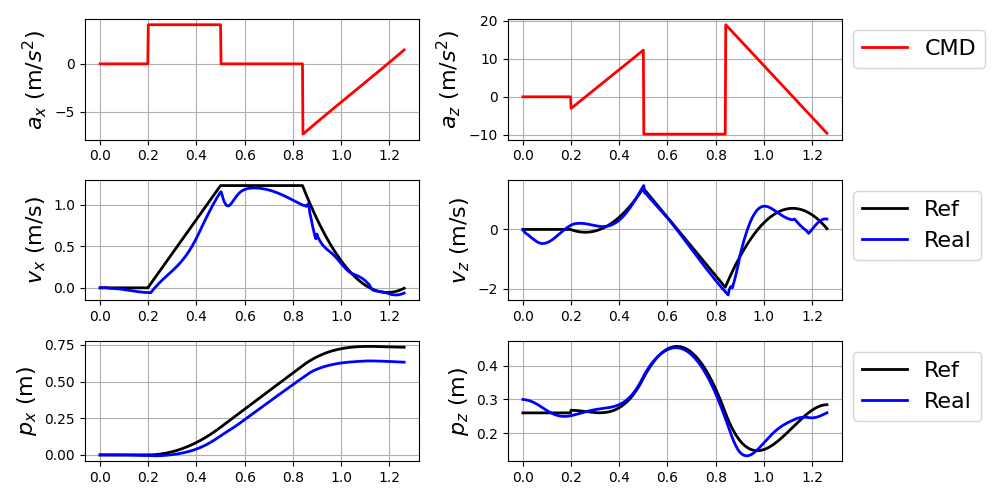
\includegraphics[width=0.85\columnwidth]{figures/jump_w_opt_tracking.png}}
        \caption{Single pronking circle with optimized transition. The position tracking MSE error is 0.0017.}
        \label{fig:jump_tracking_w_opt}
\end{figure}

\begin{figure}[htb]
    \centering
        \textsf{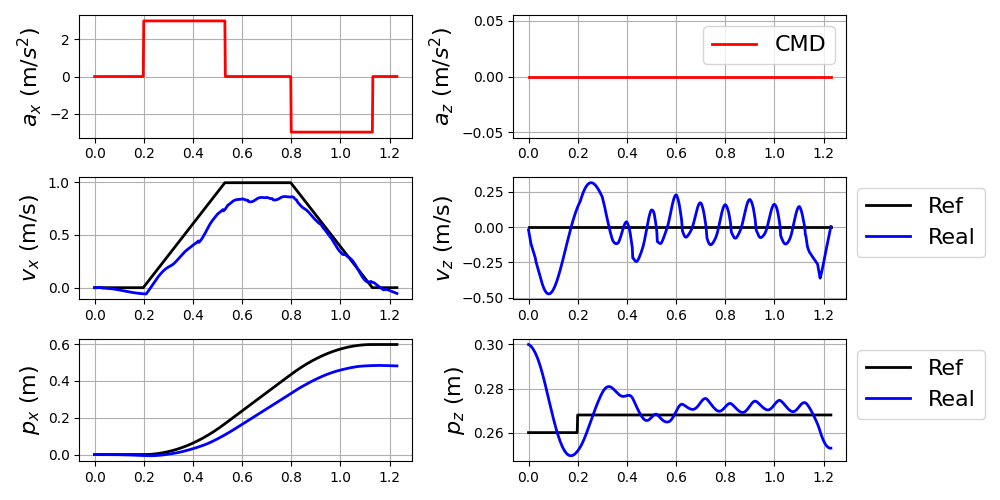
\includegraphics[width=0.85\columnwidth]{figures/trot_ref_tracking.png}}
        \caption{Single trotting circle with optimized transition. The position tracking MSE error is 0.0032.}
        \label{fig:trot_tracking}
\end{figure}


\subsection{Continuous Jumping}

\begin{figure}[H]
    \centering
        \textsf{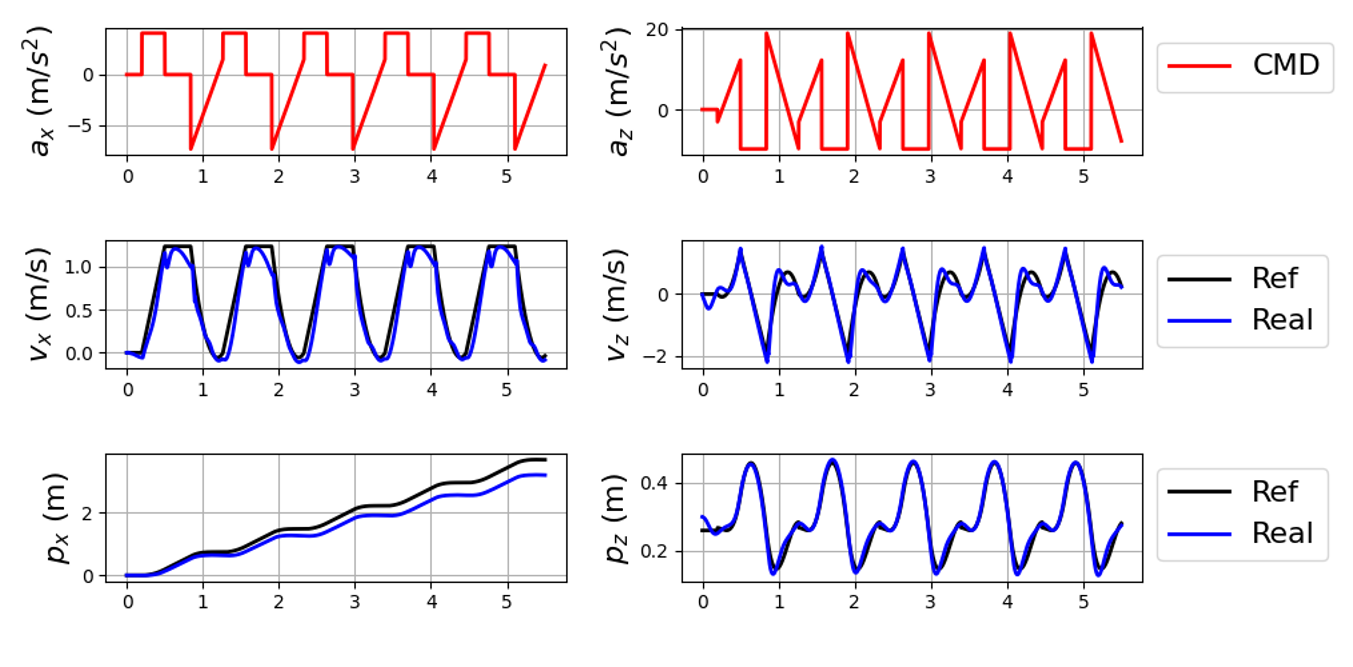
\includegraphics[width=0.9\columnwidth]{figures/continuous_jump_tracking.png}}
        \caption{Continuous jumping, \href{https://drive.google.com/file/d/1W2lfmGC67l_4fw870qR48iA-APiqXFV_/view?usp=drive_link}{video link}}
        \label{fig:continuous_jump}
\end{figure}


\subsection{Transitions between Trotting and Jumping}

\begin{figure}[H]
    \centering
        \textsf{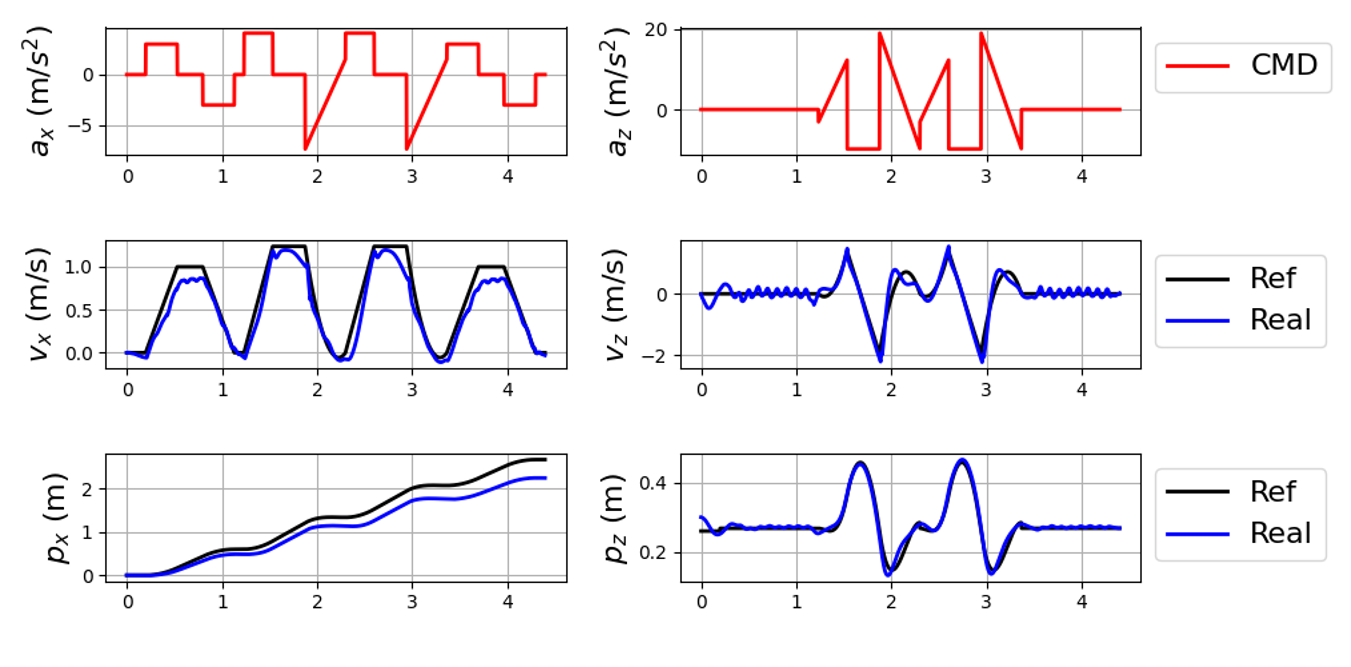
\includegraphics[width=0.9\columnwidth]{figures/mix_jump.png}}
        \caption{Transitions between trotting and jumping, \href{https://drive.google.com/file/d/1HB1HqvXQw2wybF_QYKwW6OonTc9PMxFE/view?usp=drive_link}{video link}}
        \label{fig:mix_jump}
\end{figure}


\subsection{Centroidal Policy Training}

\subsubsection{Training with reference}
\href{https://drive.google.com/file/d/1pSJmZ-tl52aZ7GZI2nzOxkKTZGH0hfcQ/view?usp=drive_link}{video link}
\begin{itemize}
    \item No good results have been obtained till the submission of this report
    \item Lessons learned: precise domain knowledge is needed to properly combine model-based method with RL, e.g. tuning hyperparameter from both sides
\end{itemize}

\subsubsection{Training without reference}
\href{https://drive.google.com/file/d/1G1joUFXv9Kfyl7xER_ZQAMzWuTytkTiu/view?usp=drive_link}{video link}
\begin{itemize}
    \item Trained surprisingly good without reference
    \item Just switched gait scheduler after each gait circle
\end{itemize}

\section{Conclusions}
In conclusion, LocoJump offers a parallelizable and extendable framework for achieving controlled versatile jumping capabilities in legged robots. Through a combination of trajectory optimization, and RL aided model-based control methods, experimental results validate the effectiveness of the proposed approach, showcasing smooth and stable transitions between different motion modes and accurate tracking of reference trajectories.

% Future works:
% \begin{itemize}
%     \item Switch the robot URDF to Unitree Go2
%     \item Implement MPC for low-level tracking
%     \item Transit gait at higher initial velocities
%     \item Jump to stairs or jump over gaps
%     \item Transit motion based on terrain types
% \end{itemize}



\FloatBarrier
% \clearpage
% \nocite{*}
\bibliographystyle{IEEEtran}
\bibliography{ref.bib}


\end{document}
